\documentclass[12pt]{article}
\usepackage[a4paper,margin=1in]{geometry}
\usepackage{amsmath,amssymb}
\usepackage{graphicx}
\usepackage{siunitx}
\sisetup{per-mode=symbol}
\usepackage{gvv}

\title{Matrix 4.8.11}
\author{ai25btech11015 -- M Sai Rithik}
\date{}

\begin{document}
\maketitle

\section*{Question}
Find the vector equation of the plane determined by the points
\[
A(3,-1,2),\quad B(5,2,4),\quad C(-1,-1,6),
\]
and hence find the distance of this plane from the origin.  


\section*{Solution}

\subsection*{Step 1: Position vectors}
\begin{equation}
\Vec{A} = \myvec{3\\-1\\2},\qquad
\Vec{B} = \myvec{5\\2\\4},\qquad
\Vec{C} = \myvec{-1\\-1\\6}.
\label{eq:points}
\end{equation}

\subsection*{Step 2: Plane as $\mathbf{N}^{\!\top}x = 1$}
Write the plane in the normalized form
\begin{equation}
\mathbf{N}^{\!\top} x = 1,
\label{eq:plane1}
\end{equation}
where \(\mathbf{N}=\myvec{n_1\\n_2\\n_3}\) is the (unknown) column vector of coefficients.  
Since \(A,B,C\) lie on the plane we must have
\begin{equation}
\mathbf{N}^{\!\top}\Vec{A} = 1,\qquad
\mathbf{N}^{\!\top}\Vec{B} = 1,\qquad
\mathbf{N}^{\!\top}\Vec{C} = 1.
\label{eq:pointconds}
\end{equation}

\subsection*{Step 3: Linear system (matrix form)}
Equations \eqref{eq:pointconds} give the linear system
\begin{equation}
\begin{bmatrix}
3 & -1 & 2\\[4pt]
5 & 2 & 4\\[4pt]
-1 & -1 & 6
\end{bmatrix}
\myvec{n_1\\n_2\\n_3}
=
\myvec{1\\1\\1}.
\label{eq:matrixsystem}
\end{equation}
We solve \eqref{eq:matrixsystem} by row reduction.  Write the augmented matrix:
\begin{equation}
\left[
\begin{array}{ccc|c}
3 & -1 & 2 & 1\\[6pt]
5 & 2 & 4 & 1\\[6pt]
-1 & -1 & 6 & 1
\end{array}
\right].
\label{eq:aug0}
\end{equation}

\subsection*{Step 4: Row reduction (RREF steps)}
Perform elementary row operations; each step is shown.

\medskip

\noindent\textbf{(i)} Eliminate the first column below the pivot in row 1:
\[
R_2 \leftarrow R_2 - \frac{5}{3}R_1,\qquad
R_3 \leftarrow R_3 + \frac{1}{3}R_1,
\]
giving
\begin{equation}
\left[
\begin{array}{ccc|c}
3 & -1 & 2 & 1\\[6pt]
0 & \dfrac{11}{3} & \dfrac{2}{3} & -\dfrac{2}{3}\\[8pt]
0 & -\dfrac{4}{3} & \dfrac{20}{3} & \dfrac{4}{3}
\end{array}
\right].
\label{eq:aug1}
\end{equation}

\medskip

\noindent\textbf{(ii)} Clear denominators in rows 2 and 3 by multiplying those rows by \(3\):
\[
R_2 \leftarrow 3R_2,\qquad R_3 \leftarrow 3R_3,
\]
so
\begin{equation}
\left[
\begin{array}{ccc|c}
3 & -1 & 2 & 1\\[6pt]
0 & 11 & 2 & -2\\[6pt]
0 & -4 & 20 & 4
\end{array}
\right].
\label{eq:aug2}
\end{equation}

\medskip

\noindent\textbf{(iii)} Eliminate the (3,2)-entry using row 2:
\[
R_3 \leftarrow R_3 + \frac{4}{11}R_2,
\]
which yields
\begin{equation}
\left[
\begin{array}{ccc|c}
3 & -1 & 2 & 1\\[6pt]
0 & 11 & 2 & -2\\[8pt]
0 & 0 & \dfrac{228}{11} & \dfrac{36}{11}
\end{array}
\right].
\label{eq:aug3}
\end{equation}

\medskip

\noindent\textbf{(iv)} Scale Row3 to make the pivot \(1\):
\[
R_3 \leftarrow \frac{11}{228}R_3,
\]
so Row 3 becomes
\begin{equation}
\left[\,0\; 0\; 1\; \big|\; \frac{36}{228}\,\right] = [\,0\;0\;1\;|\; \tfrac{3}{19}\,].
\label{eq:aug4}
\end{equation}
Thus
\begin{equation}
n_3 = \frac{3}{19}.
\label{eq:n3}
\end{equation}

\medskip

\noindent\textbf{(v)} Back substitution to clear above pivots:

Eliminate the 3rd column entry in Row2:
\[
R_2 \leftarrow R_2 - 2R_3 \quad\Longrightarrow\quad
\big[\,0\;11\;0\;|\;-2 - 2\cdot\tfrac{3}{19}\,\big] = \big[\,0\;11\;0\;|\;-\tfrac{44}{19}\,\big].
\]
Hence
\begin{equation}
11\,n_2 = -\frac{44}{19}\quad\Longrightarrow\quad
n_2 = -\frac{4}{19}.
\label{eq:n2}
\end{equation}

Eliminate the 2nd and 3rd column entries in Row1:
\[
R_1 \leftarrow R_1 + R_2 - 2R_3,
\]
which produces the equation
\begin{equation}
3\,n_1 = 1 + n_2 - 2n_3 = 1 -\frac{4}{19} - \frac{6}{19} = \frac{9}{19}.
\end{equation}
So
\begin{equation}
n_1 = \frac{3}{19}.
\label{eq:n1}
\end{equation}

\subsection*{Step 5: Plane equation and distance}
Thus the solution is
\begin{equation}
\mathbf{N} \;=\; \myvec{\dfrac{3}{19}\\[4pt] -\dfrac{4}{19}\\[4pt] \dfrac{3}{19}}.
\label{eq:Ntilde}
\end{equation}
Equivalently, scaling by \(19\),
\begin{equation}
\Vec{N} \;=\; \myvec{3\\-4\\3}, \qquad
\Vec{N}^{\!\top} x = 19,
\label{eq:Nscaled}
\end{equation}
so \eqref{eq:plane1} holds with \(\mathbf{N}\) as in \eqref{eq:Ntilde}.

The perpendicular distance \(D\) from the origin to the plane \(\mathbf{N}^{\!\top}x=1\) equals
\begin{equation}
D \;=\; \frac{|1|}{\|\mathbf{N}\|}.
\label{eq:dist1}
\end{equation}
Compute
\begin{equation}
\|\Vec{N}\| = \sqrt{3^2 + (-4)^2 + 3^2} = \sqrt{34},
\end{equation}
so, since \(\|\mathbf{N}\| = \|\Vec{N}\|/19\),
\begin{equation}
D \;=\; \frac{1}{\|\mathbf{N}\|} \;=\; \frac{19}{\sqrt{34}} \;=\; \frac{19\sqrt{34}}{34} \approx 3.260.
\label{eq:distfinal}
\end{equation}

\section*{Final Answer}
\begin{equation}
\boxed{\;\mathbf{N}^{\!\top}x = 1,\quad
\mathbf{N}=\myvec{\dfrac{3}{19}\\[4pt]-\dfrac{4}{19}\\[4pt]\dfrac{3}{19}}\;}
\end{equation}
\begin{equation}
\boxed{ \text{Distance from origin to plane} = \dfrac{19}{\sqrt{34}} \approx 3.260 }
\end{equation}

\begin{figure}[h!]
    \centering
    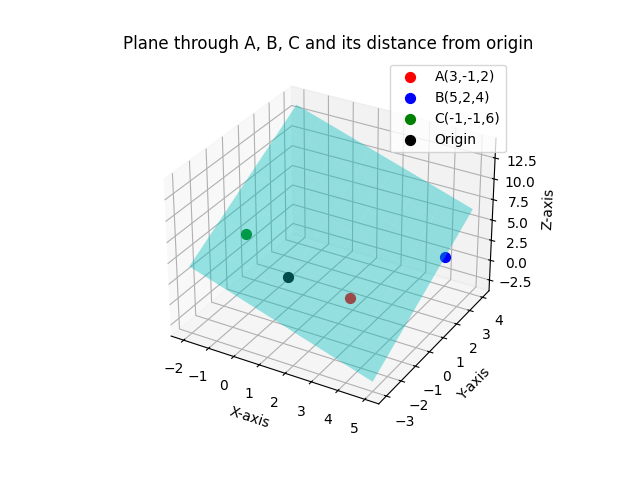
\includegraphics[width=0.65\linewidth]{figs/fig.png}
    \caption{(Sketch: plane through $A,B,C$).}
\end{figure}

\end{document}
